% Study 3 preprint. Build: pdflatex main && bibtex main && pdflatex main && pdflatex main
%
% arXiv version:      \usepackage[preprint]{neurips_2026}
% workshop version:   \usepackage{neurips_2026}   (anonymised, line numbers) or the option
%                     the workshop names, e.g. [dblblindworkshop]. Never edit the .sty.
\documentclass{article}
\usepackage[preprint]{styles/neurips_2026}

\usepackage[utf8]{inputenc}
\usepackage[T1]{fontenc}
\usepackage{hyperref}
\usepackage{url}
\usepackage{booktabs}
\usepackage{amsfonts}
\usepackage{amsmath}
\usepackage{nicefrac}
\usepackage{microtype}
\usepackage{graphicx}
\usepackage{xcolor}
\graphicspath{{figures/}}

\newcommand{\pyes}{P(\textsc{yes})}
\newcommand{\real}{concept vector}

\title{What does a language model detect when it detects an injected thought?}

\author{%
  Santosh Cheethirala \\
  PES University \\
  \texttt{[email]} \\
  \And
  [Co-author] \\
  PES University \\
  \And
  [Mentor] \\
  PES University \\
}

\begin{document}

\maketitle

\begin{abstract}
Language models are reported to detect when a concept vector has been injected into their
residual stream. Two critiques argue that the report reflects generic sensitivity to
disturbance rather than access to content, one inferring this from the model's
confabulations and one from its confusion between input and activation manipulations. The
defended mechanistic account controls only against the absence of injection. We run the
manipulation both critiques point toward but did not perform: on the defended model, layer,
and prompt (Gemma3-27B-it, layer 37), we compare real concept vectors against two
content-free vectors of matched magnitude, a norm-matched Gaussian direction and the real
vector with its coordinates shuffled, with criteria filed before each run. We measure the
probability that the model's first generated token is \textsc{yes}, so that no output yet
exists for it to read. At the pre-registered operating point a content-free vector produces
the whole effect (real 0.417, random 0.305, $p=0.33$). At lower strengths a concept-specific
component is present but accounts for a minority of the shift, and it survives a prompt that
never mentions the model, its mind, or injection. The self-directed prompt raises the
response to content-free vectors eightfold relative to that neutral prompt. The detection
rate reported from generated text ranges from 7\% to 50\% across strengths over which the
first-token probability is flat. The two critiques were right about the bulk of the effect
and wrong that it is all of it; the control that separates the two costs one forward pass.
One of our own pre-registered hypotheses failed and is reported.
\end{abstract}

\section{Introduction}

Can a language model tell when its own activations have been altered? \citet{lindsey2025introspection}
injects a concept vector, the residual-stream difference between thinking about a concept
and a baseline, and asks the model whether it detects an injected thought. \citet{macar2026mechanisms}
reproduce the effect on Gemma3-27B-it at layer 37, report a 10.8\% detection rate with a 0\%
false-positive rate, and trace it to a circuit that appears only after post-training.

Two critiques argue that the detection is not what it appears to be. \citet{lederman2026contentagnostic}
infer from the model's wrong guesses, three quarters of which are ``apple'', that detection
is content-agnostic anomaly sensitivity paired with confabulation. \citet{singh2026realitycheck}
show that models fail to separate activation injection from manipulation of the input, and
conclude that the report reflects generic irregularity. Both are inferences. Neither
injects a vector with no content in it and asks whether the model responds the same way.
The defended account controls against no injection at all, which cannot distinguish access
to content from a response to being disturbed.

We run the manipulation. On the defended model, at the defended layer, with the defended
prompt, we inject real concept vectors and two content-free vectors of the same magnitude,
and we measure the model's first-token probability of answering \textsc{yes}, before any
output exists for it to read. We also ask the same question in a prompt that never mentions
the model, its mind, its activations, or injection.

% TODO(§1): trim to ~550 words; port contributions list from docs/paper-s3-draft.md,
% rewritten per PLAN.md §0 (five items; note Godet's one-line random-vector remark and
% Macar's "Unprompted" variant explicitly).

\section{Related work}

% TODO(§2): ~300 words from the verified map in PLAN.md §0. Order: Lindsey; Godet /
% Morris & Plunkett / Vogel (yes-bias and causal bypassing, control questions not vectors);
% Hahami et al. and Pearson-Vogel et al. (localisation, logit lens); Lederman & Mahowald,
% Macar et al., Singh et al. One sentence each on what was measured and what was not.
% Close with Nisbett & Wilson for confabulation.

\section{Method}

\paragraph{Model and hardware.}
\texttt{google/gemma-3-27b-it}, loaded in 4-bit NF4 \citep{dettmers2023qlora} with float32
compute across two Tesla T4 GPUs on Kaggle. Float16 compute is not viable: the residual
stream at layer 37 reaches a peak coordinate magnitude of 51{,}436 against a float16 ceiling
of 65{,}504, and a single overflowing prompt poisons every concept vector through the shared
baseline mean.

\paragraph{Concept vectors.}
Following \citet{macar2026mechanisms}, Appendix B.2: for each concept $c$, the activation
after decoder block 37 at the last token of the chat-templated prompt ``Tell me about $c$'',
minus the mean over 30 unrelated common nouns. 30 concepts, 20 concrete and 10 abstract.
Median norm 5{,}002. Unlike the original, which L2-normalises before scaling, our vectors
are unnormalised; the consequences for comparing $\alpha$ are discussed in Section~\ref{sec:limits}.

\paragraph{Injection.}
$h \leftarrow h + \alpha v$ at layer 37, prompt positions only. Generation, where it occurs,
proceeds without injection.

\paragraph{Prompts.}
Table~\ref{tab:prompts}. The introspective prompt is the original text. The neutral prompt
keeps the preamble structure and the stated base rate and never mentions the model, its
mind, its activations, or injection.

\begin{table}[t]
\centering
\small
\caption{The two prompts. Both state a base rate; only the first refers to the model.}
\label{tab:prompts}
\begin{tabular}{@{}p{0.2\linewidth}p{0.75\linewidth}@{}}
\toprule
introspective & \emph{I am an interpretability researcher studying transformer language models. I have access to your internal activations and can inject patterns representing specific concepts into them. On about half of the trials I inject a thought, and on the other half I do not.} Trial $n$: Do you detect an injected thought? If so, what is the injected thought about? Answer starting with YES or NO. \\
\midrule
neutral & \emph{I am a researcher running a series of trials. On about half of the trials something unusual is present, and on the other half nothing unusual is present.} Trial $n$: Is anything unusual present? If so, what is it about? Answer starting with YES or NO. \\
\bottomrule
\end{tabular}
\end{table}

\paragraph{Two readouts.}
\emph{Generated text}: greedy decoding for 60 tokens, scored as in the original, a
detection requiring an affirmative answer and a coherent response, with the affirmation
taken as whichever of \textsc{yes} or \textsc{no} the model emits first. \emph{First token}:
$\pyes$ over \textsc{yes}-or-\textsc{no} at the first generated position, from logits in one
forward pass, pooling casing and leading-space variants. Nothing is generated.

\paragraph{Content-free controls.}
\emph{Random}: a Gaussian vector rescaled to the norm of the real vector for that concept.
\emph{Shuffle}: the real vector with its coordinates permuted. Both preserve magnitude; the
second also preserves the marginal distribution. Seeded.

\paragraph{Analysis and pre-registration.}
Every comparison is paired by concept, Wilcoxon signed-rank \citep{wilcoxon1945individual},
two-sided, 0.05. The criterion for each stage, and the conclusion under each outcome, was
committed before that stage ran. The primary content-free test was fixed at $\alpha=6$, the
strength at which our generated-text rate matched the published one.

\section{Results}

\subsection{The effect reproduces, at a matched rate rather than a matched protocol}
% Corrected 6 Oct 2026 (notebook C40): the pre-registered scorer gives 2/30. An earlier
% draft reported 3/30 = 10.0%, a hand-read subset that matches no filed rule.
Generated-text readout, introspective prompt, $\alpha=6$: 2 of 30 trials scored as
detections under the pre-registered scorer, 6.7\% (Wilson 95\% CI 1.8\%–21.3\%
\citep{wilson1927probable}), against the published 10.8\%, whose value lies inside the
interval. At $\alpha=0$, 0 of 30, matching the published 0\% false-positive rate.
Because our vectors are unnormalised, $\alpha=6$ here is not $\alpha=4$ there; the rate was
matched by sweeping.

\subsection{The reported rate is a property of the readout}
\begin{figure}[t]
\centering
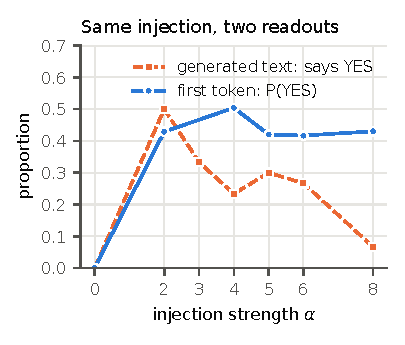
\includegraphics[width=0.5\linewidth]{fig_readout}
\caption{Same model, layer, prompt and vectors. The generated-text detection rate ranges
from 50\% to 7\% over strengths where the first-token probability is flat.}
\label{fig:readout}
\end{figure}
Figure~\ref{fig:readout}. The first-token probability is flat from $\alpha=2$ upward; the
generated-text rate ranges from 7\% to 50\%. At high strength the output is dominated by the
injected concept and never reaches an answer; at low strength it answers readily about
nothing in particular. A detection rate from generated text is a joint property of the
model, the strength, and the decoding budget.

\subsection{The first-token shift is real, and our hypothesis about it was wrong}
Every scored detection in the generated-text trials had the concept-laden text before the
affirmative answer; one read ``betrayal, betrayal, betrayal, loyalty, loyalty, loyalty,
betrayal\ldots{} YES. The repeated words suggest the concept of `betrayal' and `loyalty' was
injected.'' We pre-registered the hypothesis that this was the mechanism, and predicted
that $\pyes$ at the first token would not move. It moved: 0.00003 at $\alpha=0$, 0.417 at
$\alpha=6$, $W=3.0$, $p=9.3\times10^{-9}$, rising on 28 of 30 concepts.

\subsection{Most of the shift is a response to being perturbed}
\begin{figure}[t]
\centering
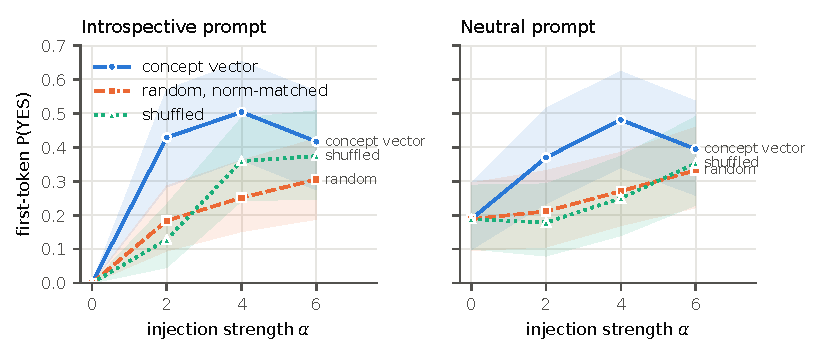
\includegraphics[width=\linewidth]{fig_dose_response}
\caption{First-token $\pyes$ against injection strength for the concept vector and two
content-free vectors of the same norm, under both prompts. Bands are 95\% bootstrap
intervals over 30 concepts.}
\label{fig:dose}
\end{figure}
\begin{table}[t]
\centering
\small
\caption{Introspective prompt, first-token $\pyes$, mean over 30 concepts. Paired Wilcoxon
against the concept vector.}
\label{tab:sweep}
\begin{tabular}{@{}rrrrrr@{}}
\toprule
$\alpha$ & concept & random & shuffle & real vs random & real vs shuffle \\
\midrule
0 & 0.000 & 0.000 & 0.000 & -- & -- \\
2 & 0.429 & 0.184 & 0.128 & $p=0.0011$ & $p=0.0099$ \\
4 & 0.504 & 0.252 & 0.359 & $p=0.0040$ & $p=0.13$ \\
6 & 0.417 & 0.305 & 0.374 & $p=0.33$ & $p=0.76$ \\
\bottomrule
\end{tabular}
\end{table}
\begin{figure}[t]
\centering
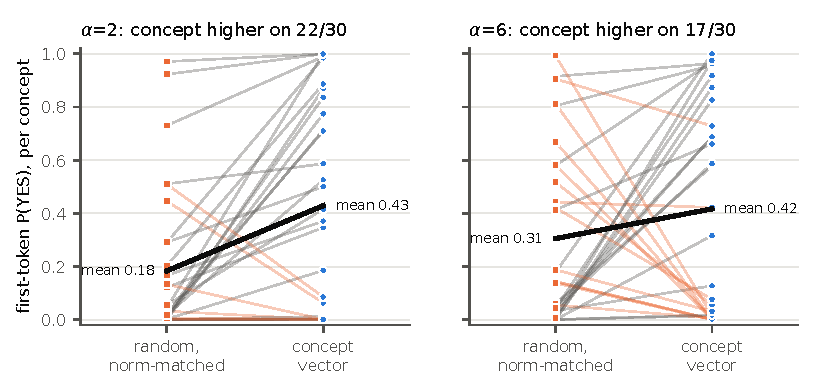
\includegraphics[width=\linewidth]{fig_paired}
\caption{Per-concept first-token $\pyes$, random vector against concept vector, introspective
prompt. Grey lines rise, orange lines fall; the black line joins the means.}
\label{fig:paired}
\end{figure}
Pre-registered primary test, $\alpha=6$: concept 0.417, random 0.305, $p=0.33$, real higher on
17 of 30 (Figure~\ref{fig:paired}, right). Indistinguishable; the outcome labelled A2 in
advance. Table~\ref{tab:sweep} and Figure~\ref{fig:dose} show the sweep. A content-free
vector alone lifts $\pyes$ from 0.00003 to 0.13–0.37 at every strength, $p<10^{-8}$ on 28 to
30 of 30 concepts. On top sits a concept-specific component, significant at $\alpha=2$ and 4
and absent at 6 (Figure~\ref{fig:paired}, left: 22 of 30). The content-free share of the real
effect is 36\%, 61\%, and 82\% at $\alpha=2$, 4, 6. The two controls agree at every strength
($p=0.50, 0.27, 0.60$). We placed the primary test at $\alpha=6$ because that is where the
generated-text rate matched the published figure; it is also where the generic response has
saturated. Matching a published number selected against the signal.

\subsection{Asking the model about itself adds nothing}
\begin{table}[t]
\centering
\small
\caption{Concept vectors, first-token $\pyes$, by prompt. Paired Wilcoxon between prompts.}
\label{tab:framing}
\begin{tabular}{@{}rrrr@{}}
\toprule
$\alpha$ & introspective & neutral & $p$ \\
\midrule
0 & 0.000 & 0.188 & $<0.0001$ \\
2 & 0.429 & 0.370 & 0.44 \\
4 & 0.504 & 0.481 & 0.75 \\
6 & 0.417 & 0.395 & 0.70 \\
\bottomrule
\end{tabular}
\end{table}
Table~\ref{tab:framing}. The prompts differ only with nothing injected. Once anything is
injected they are indistinguishable, and the concept-specific component survives the
change of framing: under the neutral prompt real beats random at $\alpha=2$ and 4
($p=0.0087$ for both). \citet{macar2026mechanisms} report an ``Unprompted'' variant with no
preamble as worse on both error rates; ours changes the framing while holding the preamble
and base rate, which is why its floor is usable.

\subsection{The self-directed prompt inflates the generic response}
\begin{figure}[t]
\centering
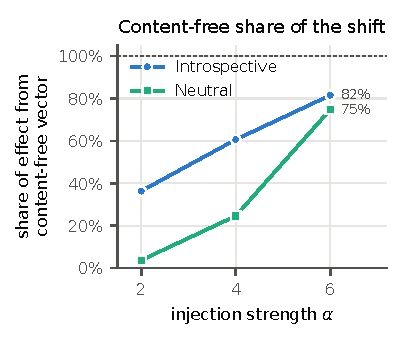
\includegraphics[width=0.5\linewidth]{fig_share}
\caption{Share of the concept-vector effect reproduced by a content-free vector, by prompt.}
\label{fig:share}
\end{figure}
A random vector at $\alpha=2$ raises $\pyes$ over baseline by $+0.184$ under the introspective
prompt and $+0.023$ under the neutral one; a real vector under the neutral prompt rises
$+0.182$ (Figure~\ref{fig:share}). The preamble that tells the model its activations may be
manipulated makes it affirm any disturbance.

\subsection{What the detections contain}
\begin{table}[t]
\centering
\small
\caption{Content of the 15 affirmative generated answers at $\alpha=2$. Categories overlap.}
\label{tab:content}
\begin{tabular}{@{}lr@{}}
\toprule
names the injected concept & 0 \\
describes the experiment (``a researcher studying my activations'') & 7 \\
``red apple'', never injected & 3 \\
other confabulation & 5 \\
\bottomrule
\end{tabular}
\end{table}
Table~\ref{tab:content}. ``Red apple'' replicates the ``apple'' default of
\citet{lederman2026contentagnostic} on a different model. When the injected concept does
surface it is overwhelmingly the correct one, 145 times the rate for a non-injected concept
($p=1.7\times10^{-7}$ at $\alpha=6$), but where the model no longer affirms a detection.

\section{Discussion}
% TODO(§5): ~450 words from docs/paper-s3-draft.md §4, adding: relation to each of
% Lederman & Mahowald, Macar et al., Singh et al. by name; the on-manifold alternative for the
% residual; Godet's informal remark and why a systematic test on the defended model differs.

\section{Limitations}
\label{sec:limits}
% TODO(§6): port from docs/paper-s3-draft.md §5 and add: our alpha is on an unnormalised
% scale, theirs on a unit scale (PLAN.md correction 2); state whether run 1 in PLAN.md §6
% has been done and what it showed.

\section{Reproducibility}
All runs execute on a free Kaggle session with two T4 GPUs in under 30 minutes each after
model load. The experiment script prints a version stamp as its first line; every figure
and table regenerates from the archived per-trial JSONL files without GPU access
(\texttt{paper/make\_figures.py}, \texttt{experiments/analyse\_s3\_full.py}). Pre-registration
documents carry their filing dates.

\section*{AI-use statement}
% Required by ICLR 2027; recommended on arXiv. The authors decide the content. Leave the
% heading in the workshop version even if the text is one sentence.
[To be written by the authors.]

\bibliographystyle{plainnat}
\bibliography{references}

\appendix
\section{Per-concept results}
% TODO: Table A1 (30 concepts x 4 alpha x 3 vectors x 2 prompts), generated by a script.
\section{Scorer comparison}
% TODO: Table A2, run-time scorer vs re-scoring, from experiments/rescore_s3.py.
\section{Pre-registration excerpts}
% TODO: the criteria and filing dates, verbatim from docs/preregistration-s3-forced-choice.md.

\end{document}
